\part{Terminal Hacking}

\begin{figure}
    \begin{center}
        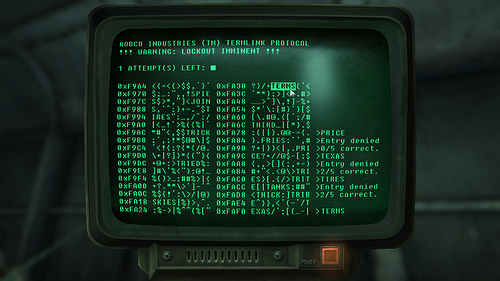
\includegraphics[width=0.8\textwidth]{fallout_terminal.jpg}
    \end{center}
    \caption{A screenshot of the hacking minigame in \emph{Fallout~4}.
    Image from \protect\url{http://fallout.wikia.com/wiki/Terminal}.}
    \label{fig:fallout_terminal}
\end{figure}

In this part, you will implement a version of the ``terminal hacking'' minigame from \emph{Fallout~4} (Bethesda, 2015); see Figure~\ref{fig:fallout_terminal}.
In this minigame you must guess a secret $n$-letter word, one of several options presented to you.
On choosing an option, you are told the \emph{likeness}: the number of letters which match the secret word (i.e.\ the same letter in the same position).
For example if the secret word is \texttt{HOUSE} and your guess is \texttt{MOUSE}, the likeness is $4$ out of $5$.
If your guess is \texttt{HOPES}, the likeness is $2$ out of $5$ (the letters \texttt{S} and \texttt{E} do not count as they are in the wrong positions).

The GitHub repository contains a project named \texttt{PartA\_TerminalHacking} for you to build upon.
This contains code to read words from a file, and choose the secret word and other words.
You will implement the rest of the game.

\section{} \label{core-a-first}

Algorithm~\ref{alg:a_likeness} takes a guessed word and the secret word, and returns the likeness score as described above.

\textbf{Implement} the algorithm as a C++ function in \texttt{TerminalHacking.cpp}, choosing appropriate data types for the parameters, return value, and any variables.

\begin{algorithm}[t]
\begin{algorithmic}
    \Procedure{GetLikeness}{guessedWord, secretWord}
        \State $\text{result} \gets 0$
        \For{$i = 0, 1, \dots, \text{secretWord.length} - 1$}
            \If{$\text{secretWord}[i] = \text{guessedWord}[i]$}
                \State increment result
            \EndIf
        \EndFor
        \State \textbf{return} result
    \EndProcedure
\end{algorithmic}
\caption{An algorithm for calculating the likeness score for the terminal hacking minigame.}
\label{alg:a_likeness}
\end{algorithm}

\section{} \label{core-a-last}

\textbf{Implement} the main loop of the game, structured
according to the flowchart shown in Figure~\ref{fig:flowchart_a}.

\begin{figure}
\begin{center}
\begin{tikzpicture}[node distance=1.5cm]
\node (start) [startstop] {Start};
\node (choosewords) [process, below of=start] {Choose secret word and other words};
\node (displaywords) [io, below of=choosewords] {Display all words};
\node (initlives) [process, below of=displaywords] {Set lives $= 4$};
\node (enterguess) [io, below of=initlives] {Enter guess};
\node (isguessvalid) [decision, below of=enterguess, yshift=-1cm] {Is guess in list of words?};
\node (guessinvalid) [io, right of=isguessvalid, xshift=3cm] {Print ``Invalid guess''};
\node (isguesscorrect) [decision, below of=isguessvalid, yshift=-1.5cm] {Is guess correct?};
\node (youwin) [io, right of=isguesscorrect, xshift=3cm] {Print ``You win!''};
\node (stopwin) [startstop, below of=youwin] {Stop};
\node (calclikeness) [process, left of=isguesscorrect, xshift=-3cm] {Calculate likeness between guess and secret word};
\node (showlikeness) [io, below of=calclikeness] {Print likeness};
\node (loselife) [process, below of=showlikeness] {Decrement lives};
\node (isdead) [decision, below of=loselife, yshift=-0.5cm] {Is lives $\leq 0$?};
\node (youlose) [io, below of=isdead, yshift=-0.5cm] {Print ``You lose!''};
\node (stoplose) [startstop, below of=youlose] {Stop};
\draw [arrow] (start) -- (choosewords);
\draw [arrow] (choosewords) -- (displaywords);
\draw [arrow] (displaywords) -- (initlives);
\draw [arrow] (initlives) -- (enterguess);
\draw [arrow] (enterguess) -- (isguessvalid);
\draw [arrow] (isguessvalid) -- node[anchor=south] {no} (guessinvalid);
\draw [arrow] (guessinvalid) |- (enterguess);
\draw [arrow] (isguessvalid) -- node[anchor=east] {yes} (isguesscorrect);
\draw [arrow] (isguesscorrect) -- node[anchor=south] {yes} (youwin);
\draw [arrow] (youwin) -- (stopwin);
\draw [arrow] (isguesscorrect) -- node[anchor=south] {no} (calclikeness);
\draw [arrow] (calclikeness) -- (showlikeness);
\draw [arrow] (showlikeness) -- (loselife);
\draw [arrow] (loselife) -- (isdead);
\draw [arrow] (isdead) -- node[anchor=east] {yes} (youlose);
\draw [arrow] (youlose) -- (stoplose);
\coordinate[left of=isdead, xshift=-0.5cm] (tmp1);
\draw [arrow] (isdead) -- node[anchor=north] {no} (tmp1) |- (enterguess);
\end{tikzpicture}
\end{center}
\caption{Flowchart for the Terminal Hacking game}
\label{fig:flowchart_a}
\end{figure}

\section{Stretch goal} \label{stretch-a}

In the skeleton project, the words are chosen at random.
This may lead to instances of the game which are unsatisfying, for example where all words
have a low likeness score with respect to the secret word.

\textbf{Design} an improved word choosing algorithm.
Present your algorithm as pseudocode and/or a flowchart in your \texttt{readme.md} file on GitHub.

\textbf{Implement} your algorithm within your C++ project.
